
\chapter{Geometry}


The word ``geometry'' comes from the ancient Greek words ``geo'' meaning Earth and ``metron'' meaning measurement.  It is probably the oldest field of mathematics, because of its usefulness in calculating  measurements of lengths, areas, and volumes of everyday objects.


The study of geometry has evolved a great deal during the last 3,000 years or so.  Like all of mathematics, what's really important in geometry  is \emph{reasoning, making sense of problems, and justifying your solutions}.  

The mathematician Henri Poincar\'e said that 
\begin{quote}
\emph{``Geometry is the art of good reasoning from bad drawings.'' }
\end{quote}
 This insight should guide your study in this chapter.  You should never trust a drawing.  You might find that one line segment \emph{appears} to be longer than another, or an angle looks like it \emph{might be} 90 degrees.  But ``appears to be'' and ``might be'' are simply not good enough.  You have to reason through the situation and figure out what you \emph{know for sure} and why you know it.




\bigskip
\bigskip

 \begin{thinkpair*}
 Reflect on your learning of geometry in the past. What is geometry really about?   Also think about these questions:
 
 \bigskip
 
 
\begin{itemize}
\item
What is a \emph{point}?\\

\item
What is a \emph{line}? A \emph{segment}? A \emph{ray}? \\

\item
What is a \emph{plane}?\\

\item
What is a \emph{circle}? \\

\item
What is an \emph{angle}? \\

\item
Which of these basic objects can be \emph{measured}?  How are they measured?  What kinds of tools are useful?
\end{itemize}
\end{thinkpair*}

\bigskip
\bigskip

\newpage

\section{Tangrams}

\emph{Tangrams} are a seven-piece geometric puzzle that dates back at least to the Song Dynasty in China (about 1100 AD).  Below you will find the seven puzzle pieces.  Make a careful copy (a photocopy or printout is best), cut out the puzzle pieces, and then use them to solve the problems in this section.  You can trace around your solutions to remember what you have done and to have a record of your work.

\begin{center}
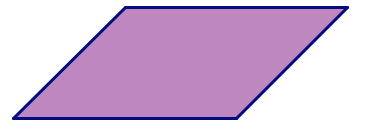
\includegraphics[scale = .470]{parallelogram}
\hfill
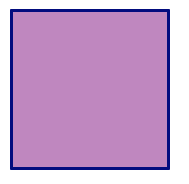
\includegraphics[scale = .470]{square}
\hfill
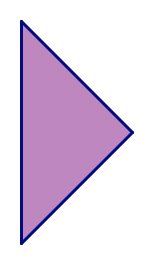
\includegraphics[scale = .470]{smtri}

\bigskip
\bigskip
\bigskip


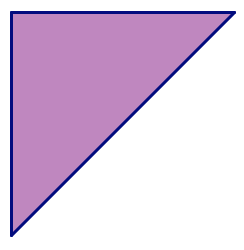
\includegraphics[scale = .470]{medtri}
\hfill
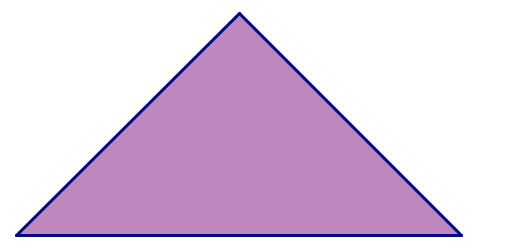
\includegraphics[scale = .470]{bigtri}

\bigskip
\bigskip


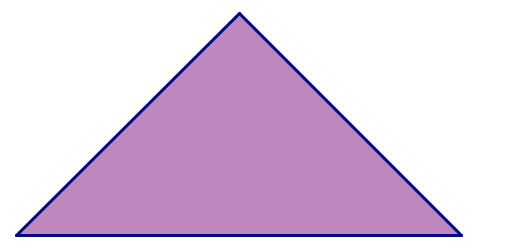
\includegraphics[scale = .470]{bigtri}
\hfill
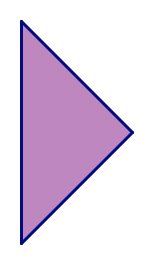
\includegraphics[scale = .470]{smtri}
\end{center}

\newpage

Whenever you solve a tangram puzzle, your job is to use all seven pieces to form the shape.  They should fit together like puzzle pieces, sitting flat on the table; no overlapping of the pieces is allowed.

\begin{problem}\label{prob:tangramsquare}
Use all seven pieces to form a square.
\end{problem}

\bigskip

\begin{problem}
Use all seven pieces to form a rectangle that is not a square.
\end{problem}

\bigskip

\begin{problem}
Use all seven pieces to form a right triangle.
\end{problem}

\bigskip

\begin{problem}
%\url{http://www.fun-stuff-to-do.com/support-files/tangram-images-variations.pdf} 
Use your tangram pieces to build the following designs.  Remember: You need to use all seven pieces, and they should fit together, not overlap.


\begin{center}
\begin{tabular}{ccc}

\includegraphics[scale=0.4]{tangram1} & 
\qquad \qquad\qquad& 

\includegraphics[scale=0.4]{tangram2}\\
(a) && (b)\\
\\
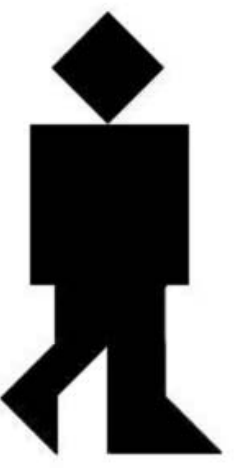
\includegraphics[scale=0.4]{tangram3} & 
\qquad \qquad\qquad& 

\includegraphics[scale=0.4]{tangram4}\\
(c) && (d)\\
\\
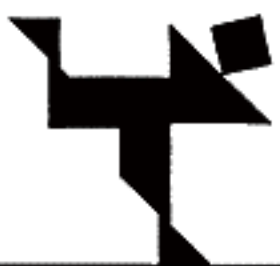
\includegraphics[scale=0.7]{tangram5} & 
\qquad \qquad\qquad& 

\includegraphics[scale=0.7]{tangram6}\\
(e) && (f)\\
\end{tabular}
\end{center}
\end{problem}

\bigskip

\begin{thinkpair*}
Which tangram problems were easier and which were harder: making ``real life'' objects like cats and people, or purely mathematical objects like the square?  What do you think made one kind of problem easier or harder?
\end{thinkpair*}

\newpage

\section{Triangles and Quadrilaterals}


\begin{thinkpair*}
Follow these directions on your own:
\begin{itemize}
\item
Draw any triangle on your paper.\\
\item
Draw a second triangle that is different in some way from your first one. Write down a sentence or two to say how it is different.\\
\item
Draw a third triangle that is different from both of your other two. Describe how it is different.\\
\item
Draw two more triangles, different from all the ones that came before.

\end{itemize}
Compare your triangles and descriptions with a partner.
To make ``different'' triangles, you have to change some feature of the triangle. Make a list of the features  that 
you or your partner changed.

\end{thinkpair*}

\newpage

Triangles are classified according to different properties.  The point of learning geometry is not to learn a lot of vocabulary, but it's useful to use the correct terms for objects, so that we can communicate clearly.  Here's a quick dictionary of some types of triangles.

\bigskip
\bigskip

\begin{center}


\begin{tabular}{c|c|c}\hline
\multicolumn{3}{c}{\bf Classification by Sides}\\
\hline\hline
{\bf scalene} & {\bf isosceles} & {\bf equilateral }  \\
\hline
all sides have  & two sides have  & all three sides have \\
different lengths & the same length & the same length\\
\hline
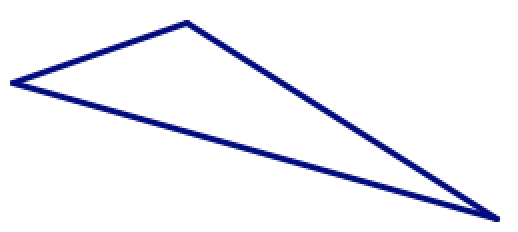
\includegraphics[height=2.5cm]{scalene} & 
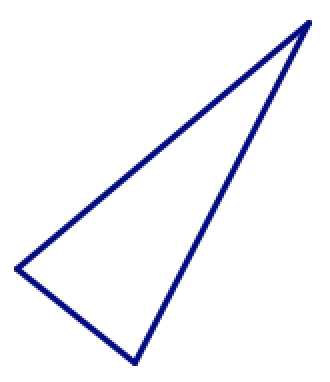
\includegraphics[height=2.5cm]{isos} &
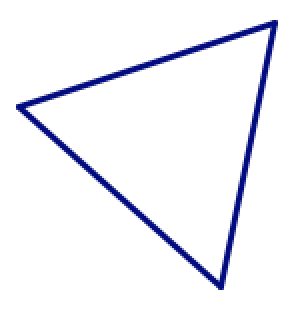
\includegraphics[height=2.5cm]{equilat}  \\
\hline\label{def:trisides}
\end{tabular}


\bigskip
\bigskip
\bigskip


\begin{tabular}{c|c}\hline
\multicolumn{2}{c}{\bf Classification by Angles}\\
\hline\hline
{\bf acute} & {\bf obtuse} \\
\hline
all interior angles   & one interior angle   \\
measure less than $90^\circ$ &  measures more than $90^\circ$ \\
\hline
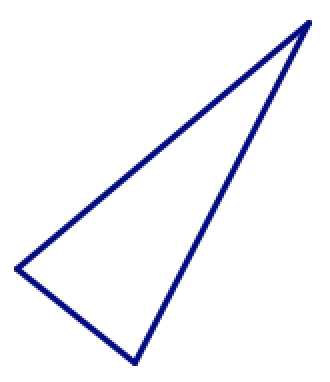
\includegraphics[height=2.5cm]{isos} & 
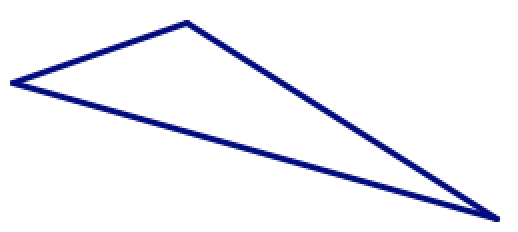
\includegraphics[height=2.5cm]{scalene}  \\
\hline
\end{tabular}

\smallskip

\begin{tabular}{c|c}\hline\label{def:triangs}
{\bf right } & {\bf equiangular} \\
\hline
 one interior angle  & all interior angles \\
 measures exactly $90^\circ$ & have the same measure\\
\hline
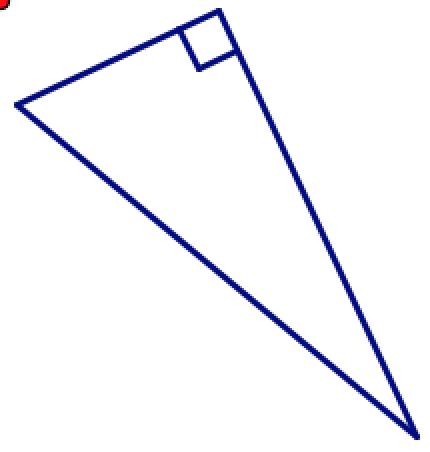
\includegraphics[height=3.5cm]{rttri} & 
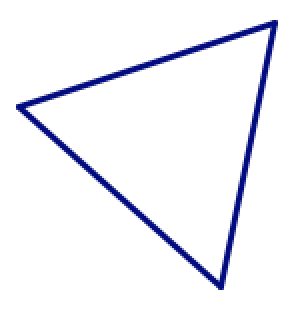
\includegraphics[height=3.5cm]{equilat}  \\
\hline
\end{tabular}

\end{center}


\newpage



Remember that ``geometry is the art of good reasoning from bad drawings.'' That means you can't always trust your eyes.  If you look at a picture of a triangle and one side \emph{looks like} it's longer than another, that may just mean the drawing was done a bit sloppily.

Mathematicians either write down measurements or use \emph{tick marks} to indicate when sides and angles are supposed to be equal.  If two sides have the same measurement attached or the same number of tick marks, you must believe they are equal and work out the problem accordingly, even if it doesn't look that way to your eyes.  One example of these marks is the little square used to indicate a right angle in the picture above.  Here are some other examples.

\bigskip



\begin{center}
\begin{tabular}{c|c}\hline
{\bf two angles equal } & {\bf two sides equal} \\
\hline
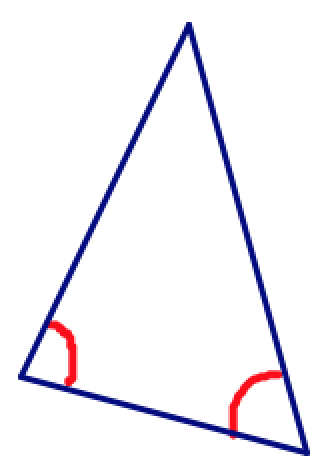
\includegraphics[height=3cm]{2eqangs} & 
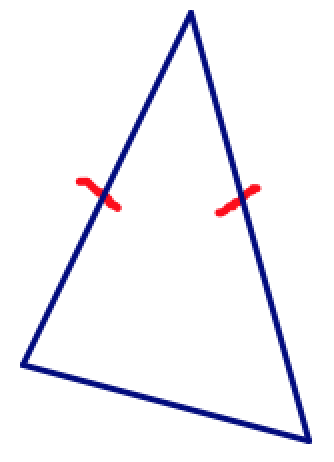
\includegraphics[height=3cm]{2eqsides}  \\
\hline
\end{tabular}

\end{center}



\bigskip
\bigskip


\subsection*{On Your Own}
Work on these exercises on your own or with a partner.  
\begin{enumerate}
\item
In the picture below, which sides are understood to have the same length?
\begin{center}
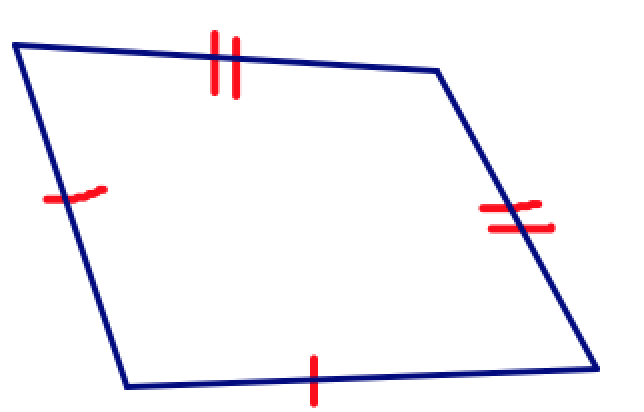
\includegraphics[height=2.5cm]{whatseq}  
\end{center}

\item
In the picture below, which angles are understood to have the same measure?
\begin{center}
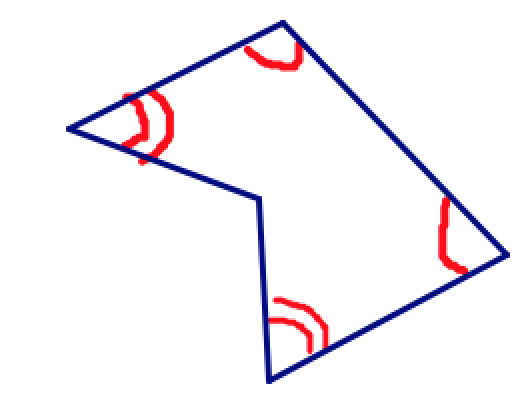
\includegraphics[height=3.7cm]{whatseq2}  
\end{center}


\item
Sketch two more scalene triangles, each of which is different from the one shown on page~\pageref{def:trisides} in some way.  \\
\item
Sketch two more acute triangles, each of which is different from the one shown on page~\pageref{def:triangs} in some way.\\
\item
Sketch two more obtuse triangles, each of which is different from the one shown on page~\pageref{def:triangs} in some way.\\
\item
Sketch two more right triangles, each of which is different from the one shown on page~\pageref{def:triangs} in some way.  Be sure to indicate which angle is $90^\circ$.\\
\item
Sketch two more isosceles triangles, each of which is different from the one shown on page~\pageref{def:trisides} in some way.  Use tick marks to indicate which sides are equal.
\end{enumerate}


\newpage


\subsection{Angle sum}

\begin{thinkpair*}
By now, you have drawn several different triangles on your paper.  Choose one of your triangles, and follow these directions:
\begin{itemize}
\item
Using scissors, cut the triangle out.  \\
\item
Tear (do not cut) off the corners, and place the three vertices together.  Your should have something that looks a bit like this picture:\\
\begin{center}
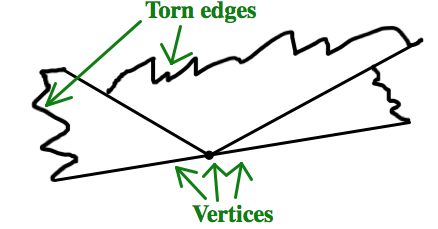
\includegraphics[height=3cm]{anglesum}
\end{center}
\fellow{This might make a nice animation, tearing off the corners and arranging them in this way.}
\end{itemize}
  What do you notice?  What does this suggest about the angles in a triangle? 
  \end{thinkpair*}
  
  
  
\bigskip
\bigskip
\bigskip

You may remember learning that the sum of the angles in any triangle is $180^\circ$.  Depending on how many students are in your class, you now have maybe 10--20 \emph{examples} of triangles where the sum of the angles \emph{seems to be} $180^\circ$.  But remember, our drawings are not exact.  How can we be sure that our eyes are not deceiving us?  How can we be sure that the sum of the angles in a triangle isn't   $181^\circ$ or $178^\circ$, but is really $180^\circ$ on the nose in every case?

\bigskip
\bigskip

\begin{thinkpair*}
What would convince you {\bf beyond all doubt} that the sum of the angles in any triangle is $180^\circ$?  Would testing lots of cases be enough?  How many is enough?  Could you ever test \emph{every possible triangle}?
\end{thinkpair*}

\newpage

\fellow{add a picture of Euclid here?}
In about 300BC, Euclid was the first mathematician (as far as we know) who tried to write down careful \emph{axioms} and then build from those axioms rigorous proofs of mathematical truths.  He had five axioms for geometry, the first four of which seemed pretty obvious to mathematicians.  People felt they were reasonable assumptions from which to build up geometric truths:
\begin{enumerate}
\item
Given two points, you can connect them with a straight line segment.\\
\item
Given a line segment, you can extend it as far as you like in either direction, making a line.\\
\item
Given a line segment, you can draw a circle having that segment as a radius.\\
\item
All right angles are congruent.\\
\end{enumerate}
The fifth postulate bothered people a bit more. It was originally stated in more flowery language, but it was equivalent to this statement:

\begin{enumerate}
\addtocounter{enumi}{4}
\item
The sum of the angles in a triangle is $180^\circ$.\\
\end{enumerate}

Often high school geometry teachers prove the sum of the angles in a triangle is $180^\circ$, usually using some facts about parallel lines.  But (maybe surprisingly?) it's just as good to take this as an \emph{axiom}, as a given fact about how geometry works, and go from there.  Perhaps this is less satisfying than proving it from some other statement, and if you're curious you can certainly find a proof or your instructor can share one with you.


It's easy to see  why this fifth axiom caused such a ruckus in mathematics.  It seemed much less obvious than the other four, and mathematicians felt like they were somehow cheating if they just \emph{assumed} it rather than \emph{proving} it had to be true.  
Many mathematicians spent many, many years trying to prove this fifth axiom from the other axioms, but they couldn't do it.  And with good reason: There are other kinds of geometries where the first four axioms are true, but the fifth one is not!  

For example, if you do geometry on a \emph{sphere} --- like a basketball or more importantly on the surface of the Earth --- rather than on a flat plane, the first four axioms are true.  But  triangles are a little strange on the surface of the earth.  Every triangle you can you can draw on the surface of the earth has an angle sum strictly greater than $180^\circ$.     In fact, you can draw a triangle on the Earth that has three right angles, making an angle sum of $270^\circ$.  

\fellow{I would really like this to be a better picture.  Maybe just a sphere with a triangle drawn on it, not a globe.  It would be nice if the right angles were marked.}

\begin{center}
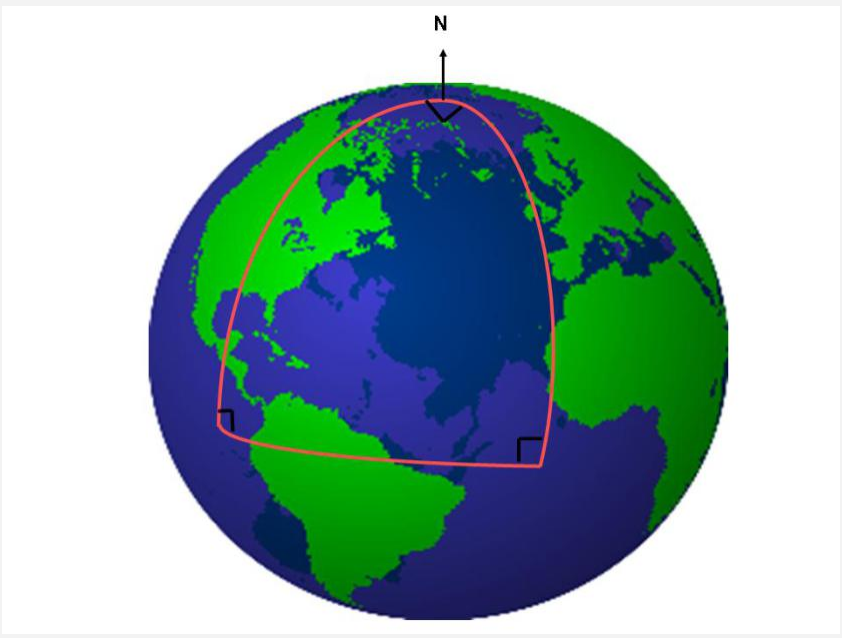
\includegraphics[height=5cm]{earthtri}
\end{center}
On a sphere like the Earth, the angle sum is not constant among all triangles.  Bigger triangles have bigger angle sums, and smaller triangles have smaller angle sums, but even the small triangles have angle sums that are greater than $180^\circ$.


The geometry you study in school is called \emph{Euclidean geometry}; it is the geometry of a flat plane, of a flat world.  It's a pretty good approximation for the little piece of the Earth that we see at any given time, but it's not the only geometry out there!


\newpage

\subsection{Triangle inequality}
Make a copy of these strips of paper and cut them out.  They have unit lengths from 1 unit to 6 units.  You may want to color them, write numbers on them, or do something that makes it easy to keep track of the different units.



\begin{center}

\includegraphics{1in}
\qquad

\includegraphics{1in}
\qquad

\includegraphics{1in}

\bigskip



\includegraphics{2in}


\includegraphics{2in}


\includegraphics{2in}



\bigskip


\includegraphics{3in}


\includegraphics{3in}


\includegraphics{3in}


\bigskip


\includegraphics{4in}


\includegraphics{4in}


\includegraphics{4in}


\bigskip


\includegraphics{5in}
 
 
\includegraphics{5in}


\includegraphics{5in}

\bigskip


\includegraphics{6in}
 
 
\includegraphics{6in}


\includegraphics{6in}
\end{center}

\newpage

\begin{problem}
Repeat the following process several times (at least 10) and keep track of the results (a table has been started for you on the next page):
\begin{itemize}
\item
Pick three  strips of paper.  (The lengths do not have to be all different from each other; that's why you have multiple copies of each length.)\\
\item
Try to make a triangle with those three strips, and decide if you think it is possible or not.  (Don't overlap the strips, cut them, or fold them.  The length of the strips should be the length of the sides of the triangle.)
\end{itemize}
Your goal is to come up with a {\bf rule} that describes when three lengths will make a triangle and when they will not. Write down the rule in your own words.
\end{problem}


\bigskip
\begin{center}
\begin{tabular}{|c c c c|}\hline
length 1 & length 2 & length 3 & triangle? \\ \hline\hline
4 & 3 & 2 & yes \\ \hline
4 & 2 & 1 & no \\ \hline
\end{tabular}
\end{center}

\bigskip
\bigskip
\bigskip


\begin{thinkpair*}
Compare your rule with other students.  
Then use your rule to answer the following questions.
\begin{itemize}
\item
Suppose you were asked to make a triangle with sides 40 units, 40 units, and 100 units units long. Do you think you could do it? Explain your answer. Keep in mind the goal is not to try to build the triangle, but to predict the outcome.\\
\item
Suppose you were asked to make a triangle with sides 2.5 units, 2.6 units, and 5 units units long. Do you think you could do it? Explain your answer. Keep in mind the goal is not to try to build the triangle, but to predict the outcome.
\end{itemize}
Of course, we know that in geometry we should not believe our eyes.    You need to look for an \emph{explanation}.  Why does your statement make sense?

\end{thinkpair*}

\newpage


You probably came up with some version of this statement:
\begin{center}
{\bf Triangle Inequaltiy}

The sum of the lengths of two sides in a triangle is \\
greater than the length of the third side.
\end{center}

\bigskip

Remember  that   ``geometry is the art of good reasoning from bad drawings.''  Our materials weren't very precise, so how can we be sure this rule we've come up with is is correct?  

Well in this case, the rule is really just the same as the saying ``the shortest distance between two points is a straight line.''  In fact, this is exactly what we mean by the words \emph{straight line} in geometry.  



\newpage

\subsection{SSS Congruence}
We say that two triangles (or any two geometric objects) are \emph{congruent} if they are exactly the same shape and the same size.  That means that if you could pick one of them up and move it to put down on the other, they would exactly overlap.

\begin{problem}\label{prob: SSS}
Repeat the following process several times and keep track of the results.
\begin{itemize}
\item
Pick three  strips of paper that will definitely form a triangle. \\
\item
Try to make two different (non-congruent) triangles with the same three strips of paper.  Record if you were able to do so.
\end{itemize}
\end{problem}

\bigskip

\begin{problem}\label{prob: noSSSS}
Repeat the following process several times and keep track of the results.
\begin{itemize}
\item
Pick four  strips of paper and form a quadrilateral with them.  (If your four strips do not form a quadrilateral, pick another four strips.)\\ 
\item
Try to make two different (non-congruent) quadrilateral with the same four strips of paper.  Record if you were able to do so.
\end{itemize}
\end{problem}


\bigskip
\bigskip

\begin{thinkpair*}
What do you notice from Problems~\ref{prob: SSS} and~\ref{prob: noSSSS}?  Can you make a general statement to describe what's going on?  Can you explain why your statement makes sense?
\end{thinkpair*}

\newpage

You probably came up with some version of this statement:
\begin{center}
{\bf SSS (side-side-side) Congruence}

If two triangles have the same side lengths,\\
then the triangles are congruent.
\end{center}

\bigskip

This most certainly is \emph{not} true for quadrilaterals.  For example, if you choose four strips that are all the same length, you can make a square:

\begin{center}

\includegraphics[scale = .45]{square2}
\end{center}
But you can also squish that square into a non-square rhombus.  (Try it!)

\begin{center}

\includegraphics[scale = .45]{square2}
\qquad\qquad
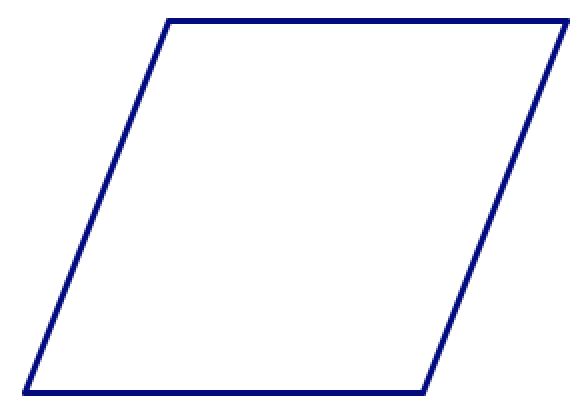
\includegraphics[scale = .45]{rhomb1}

\bigskip
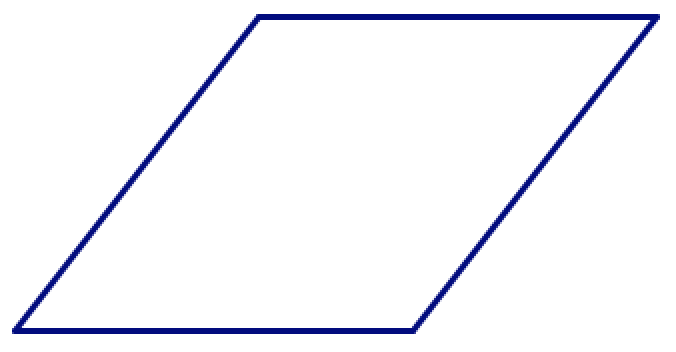
\includegraphics[scale = .45]{rhomb2}
\qquad
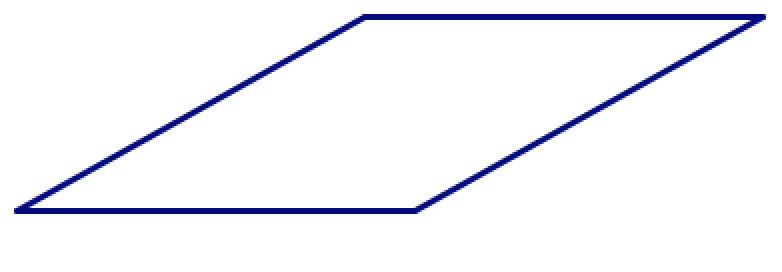
\includegraphics[scale = .45]{rhomb3}
\end{center}

If you don't choose four lengths that are all the same, in addition to ``squishing'' the shape, you can rearrange the sides to make different (non-congruent) shapes.  (Try it!)

\begin{center}
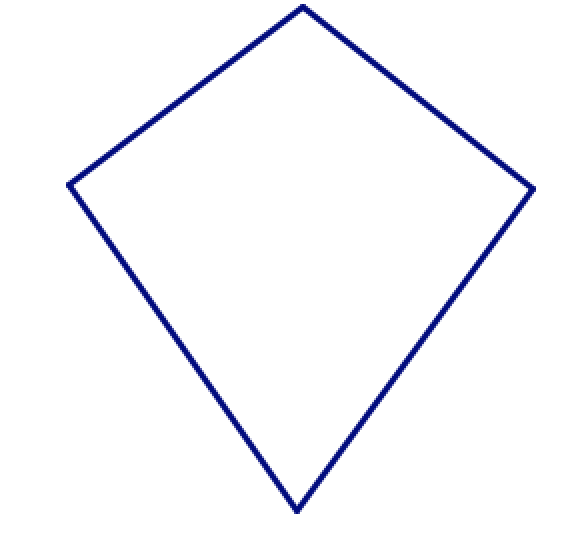
\includegraphics[scale = .45]{kite1}
\qquad\qquad
\includegraphics[scale = .45]{kite2}\\
 These two shapes have the same four side lengths in the same order.

\bigskip
\includegraphics[scale = .45]{pgram1}
\qquad
\includegraphics[scale = .45]{pgram2}\\
These two shapes have the same four side lengths as the shapes above, but the sides are in a different order.
\end{center}

\bigskip

But this can't happen with triangles.  Why not?  Well, certainly you can't rearrange the three sides.  That would be just the same as rotating the triangle or flipping it over, but not making a new shape.

Why can't the triangles ``squish'' the way a quadrilateral (and other shapes) can?  Here's one way to understand it.  Imagine you pick two of your three lengths and lay them on top of each other, hinged at one corner.



\begin{center}
\includegraphics[scale = .4]{hinge}\\
 This shows a longer purple dashed segment and a shorter green segment.  The two segments are hinged at the red dot on the left.
\end{center}
Now imagine opening up the hinge a little at a time.

\begin{center}
\includegraphics[scale = .4]{open1}
 \includegraphics[scale = .4]{open2}
 \includegraphics[scale = .4]{open3}

\includegraphics[scale = .4]{open4}
\quad
\includegraphics[scale = .4]{open5}

\includegraphics[scale = .4]{open6}
\quad
\includegraphics[scale = .4]{open7}
\end{center}

\fellow{This is almost certainly better done as an animation!}

As the hinge opens up, the two non-hinged endpoints get farther and farther apart.  Whatever your third length is (assuming you are actually able to make a triangle with your three lengths), there is {\bf exactly one} position of the hinge where it will just exactly fit to close off the triangle.  No other position will work.






\newpage

\section{Polygons}
It can seem like the study of geometry in elementary school is nothing more than learning a bunch of definitions and then classifying objects.  In this chapter, you'll explore some problem solving and reasoning activities that are based in geometry.  But definitions are still important!  So let's start with this one.

\bigskip

\begin{define}
A {\bf polygon} is:
\begin{enumerate}
\item
 a \emph{plane} figure
 \item
  that is bounded by a finite number of \emph{straight line segments}
  \item
  in which each segment \emph{meets exactly two others}, one at each of its endpoints.
\end{enumerate}
\end{define}

\bigskip

\begin{thinkpair*}
Just as the first step in problem solving is to \emph{understand the problem}, the first step in reading a mathematical definition is to \emph{understand the definition}.   
\begin{itemize}
\item
Use the definition above to draw several examples of figures that are definitely polygons.  (You should be able to say why your example fits the definition.)\\
\item
Draw several non-examples as well: shapes that are definitely not polygons.  (You should be able to say which part of the definition fails for your non-examples.)\\

\end{itemize}
\end{thinkpair*}



\newpage




A few comments about polygons:
\begin{itemize}
\item
The line segments that make up a polygon are called its \emph{edges} and the points where they meet are called its \emph{vertices} (singular: vertex).\\

\item
Because of properties (2) and (3) in the definition, the boundaries of polygons are not \emph{self-intersecting}.\\

\begin{center}
\includegraphics[scale=0.35]{notpoly} \\
Not a polygon.\\
\end{center}

\item
Polygons are named based on the number of sides they have.
\begin{center}
\begin{tabular}{c | c | c}
{\bf name} & {\bf \# of sides} & {\bf examples}\\
\hline\hline
triangle & 3 & 
\includegraphics[scale=0.5]{triex} \\
\hline
quadrilateral & 4 & 
\includegraphics[scale=0.5]{quadex} \\
\hline
pentagon & 5 & 
\includegraphics[scale=0.5]{pentex} \\
\hline
hexagon & 6 &
\includegraphics[scale=0.5]{hexex} \\
\hline
heptagon & 7 &\\
octagon & 8 & \\
nonagon & 9 & \\
decagon & 10 & 
\end{tabular}

\end{center}

\bigskip

\item
In general, we call a polygon with $n$ sides an  $n$-gon.
\end{itemize}

\bigskip


\newpage

\begin{problem}
In the pictures below, there are polygons hidden in the design.  In each design, find \emph{all} of the triangles, quadrilaterals, pentagons, and hexagons.  How can you be sure you've found them all and haven't counted any twice?

\end{problem}

\begin{center}
\includegraphics[scale=0.65]{design1} \\
Design 1

\bigskip
\includegraphics[scale=0.65]{design2} \\
Design 2

\bigskip

\includegraphics[scale=0.65]{design3} \\
Design 3

\bigskip

\includegraphics[scale=0.6]{design4} \\
Design 4


\end{center}

\newpage

\subsection{Angle sum}
You know that the sum of the interior angles in any triangle is $180^\circ$.  Can you say anything about the angles in other polygons?  
You probably know that rectangles have four $90^\circ$ angles.  So {\bf if} if all quadrilaterals have the same interior angle sum, it must be $4 \cdot 90^\circ = 360^\circ$.  

But notice: We don't necessarily have any reason to believe this constant sum would be true.  Remember that SSS congruence is true for triangles, but not for any other polygons.  Triangles are special, and we shouldn't \emph{assume} that similar statements will hold for other shapes.


\bigskip
\bigskip

\begin{thinkpair*}
Any quadrilateral can be split into two triangles, where the vertices of the triangles all coincide with the vertices of the quadrilateral:

\begin{center}
\includegraphics[height=2.9cm]{splitquads}
\end{center}
Use the pictures above to carefully explain why all quadrilaterals do, indeed, have an angle sum of $360^\circ$.

\end{thinkpair*}


\bigskip

\subsection*{On Your Own}
Work on the following exercises on your own or with a partner.
\begin{enumerate}
\item
Draw several different \emph{pentagons} on your paper.  Show that each of them can be split into exactly three triangles in such a way that the vertices of the triangles all coincide with the vertices of the pentagon.\\

\item
Use the fact that every pentagon can be split into three triangles in this way to find the sum of the angles in any pentagon.\\

\item
Draw several different \emph{hexagons} on your paper.  Show that each of them can be split into exactly four triangles so that the vertices of the triangles all coincide with the vertices of the hexagon.\\

\item
Use the fact that every hexagon can be split into four triangles in this way to find the sum of the angles in any hexagon.\\

\end{enumerate}

\bigskip
\bigskip

\newpage

\begin{problem}
Use your work on the exercises above to complete this general statement:
\begin{center}
{\bf Angle Sum in Polygons:}\\
The sum of the interior angles in an $n$-gon (a polygon with $n$ sides) is \\
\bigskip
\underline{\hskip 4 in }
\end{center}
Explain how you know this statement is true.
\end{problem}


\bigskip
\bigskip


\begin{define}
A {\bf regular polygon} has all sides the same length and all angles the same measure.  
\end{define}

For example, squares are regular quadrilaterals --- all four sides are the same length, and all four angles measure $90^\circ$.  But  a non-square rectangle is \emph{not regular}.  Even though all of the angles are $90^\circ$, the sides are not all the same length.  Similarly,  a non-square rhombus is \emph{not regular}.  Even though the sides of a rhombus are all the same length, the angles can be different.  

\begin{center}
\includegraphics[height=3cm]{regnotreg}
\end{center}

\bigskip

\begin{problem}
Since a square is a regular quadrilateral, you know that every angle in a regular quadrilateral measure $90^\circ$.  What about angles in other regular polygons?

\begin{enumerate}[(a)]
\item
What is the measure of each angle in a regular triangle?  Explain how you know you are right.\\

\item
What is the measure of each angle in a regular pentagon?  Explain how you know you are right.\\

\item
What is the measure of each angle in a regular hexagon?  Explain how you know you are right.\\

\item
What is the measure of each angle in a regular $n$-gon?  Explain how you know you are right.\\
\end{enumerate}
\end{problem}


\newpage


\section{Platonic Solids}
Of course, we live in a three-dimensional world (at least!), so only studying flat geometry doesn't make a lot of sense.  Why not think about some three-dimensional objects as well?

\bigskip

\begin{define}
A {\bf polyhedron} is as solid (3-dimensional) figure bounded by polygons.    A polyhedron has flat polygons for {\bf faces}, straight {\bf edges} where the faces meet in pairs, and {\bf vertices} where three or more edges meet.  The plural of polyhedron is {\bf polyhedra}.
\end{define}

\bigskip

\begin{thinkpair*}
Look at the pictures of solids below, and decide which are polyhedra and which are not.  You should be able to say why each figure does or does not fit the defition.
\end{thinkpair*}

\begin{center}
\begin{tabular}{ccc}
\quad
\includegraphics[height=3cm]{triprism}
\quad
&
\quad
\includegraphics[height=3cm]{cylinder}
\quad
&
\quad
\includegraphics[height=3cm]{icosahedron}
\quad\\
(a) & (b) & (c)\\
\\
\quad
\includegraphics[height=3cm]{cone}
\quad
&
\quad
\includegraphics[height=3cm]{pentantiprism}
\quad
&
\quad
\includegraphics[height=3cm]{soccerball}
\quad\\
(d) & (e) & (f)\\
\\
\quad
\includegraphics[height=3cm]{sphere}
\quad
&
\quad
\includegraphics[height=3cm]{torus}
\quad
&
\quad
\includegraphics[height=3cm]{stella}
\quad\\
(g) & (h) & (i)\\
\end{tabular}

\end{center}

\newpage

Remember that a  \emph{regular polygon} has all sides the same length and all angles the same measure.    
There is a similar (if slightly more complicated) notion of \emph{regular} for solid figures.


\begin{define}
A {\bf regular polyhedron} has  faces that are all  \emph{identical (congruent) regular polygons}.  All vertices are also identical (the same number of faces meet at each vertex).  These are called {\bf Platonic solids} (named for Plato).
\end{define}

If you fix the number of sides and their length, there is one and only one regular polygon with that number of sides.  That is, every regular quadrilateral is a square, but there can be different sized squares.  Every regular octagon looks like a stop sign, but it may be scaled up or down.  Your job in this section is to figure out what we can say about regular polyhedra.


\subsection*{On Your Own}
Work on these exercises on your own or with a partner.  You will need to make lots of copies of the regular polygons below.  Copy and cut out at least:
\begin{itemize}
\item
40 copies of the equilateral triangle,
\item
15 copies of the square,
\item
20 copies of the regular pentagon, and
\item
10 copies each of the regular hexagon, heptagon, and octagon.
\end{itemize}
You will also need some tape.


\begin{center}
\includegraphics{eqtri}

\includegraphics{square3}

\includegraphics{pentagon}

\includegraphics[scale = .75]{hexagon}

\includegraphics[scale = .75]{heptagon}

\includegraphics[scale = .75]{octagon}

\end{center}


\begin{enumerate}
\item
In any polyhedron, at least three polygons meet at each vertex.  Start with the equilateral triangles: Put three of them together meeting at a vertex and tape them together.  Then close them up so they form a solid shape.  Can you complete this into a platonic solid?  Be sure to check that at every vertex you have exactly three triangles meeting.\\

\fellow{An animation would really help here.  Students had trouble understanding the directions, but once they see it they know what to do.  Just show putting three triangles meeting at a vertex and then closing up the gap.}

\item
Now repeat this process, but start with \emph{four} equilateral triangles around a single vertex.  Then close them up so they form a solid shape.  Can you complete this into a platonic solid?  Be sure to check that at every vertex you have exactly four triangles meeting.\\

\fellow{Another animation?}


\item
Repeat this process with five equilateral triangles, then six, then seven, and so on.  Keep going until you are convinced you understand what's happening with Platonic solids that have triangular faces.\\

\item
When you are done with triangular faces, move on to square faces. Work systematically: Try  to build a Platonic solid with three squares at each vertex, then four, then five, etc.  Keep going until you can make a definitive statement about Platonic solids with square faces.\\

\item
Repeat this process with the other regular polygons you cut out: pentagons, hexagons, heptagons, and octagons.  
\end{enumerate}

\bigskip
\bigskip


You must have noticed that the situation for Platonic solids is quite different from the situation for regular polygons.  There are infinitely many regular polygons (even if you don't account for size).  There is a regular polygon with $n$ sides for every value of $n$ bigger than 2.  But for solids, we have the following (perhaps surprising) result.

\begin{thm*}
There are exactly five platonic solids.
\end{thm*}
The key fact is that for a three-dimensional solid to close up and form a polyhedron, there must be less than $360^\circ$ around each vertex.  Otherwise, it either lies flat or folds over on itself.

\bigskip

\begin{problem}
Based on your work in the exercises, you should be able to write a convincing justification of the Theorem above.  Here's a sketch, and you should fill in the explanations.  

\begin{enumerate}[(a)]
\item
If a Platonic solid has equilateral triangles for faces, then fewer than 6 faces must meet at each vertex.  Why?\\

\item
If a Platonic solid has square faces, then three faces can meet at each vertex, but not more than that.  Why?\\

\item
If a Platonic solid has regular pentagons for faces, then three faces can meet at each vertex, but not more than that.  Why?\\

\item
Regular hexagons cannot be used as the faces for a Platonic solid.  Why?\\

\item
Similarly, regular $n$-gons for $n$ bigger than 6 cannot be used as the faces for a Platonic solid.  Why?\\

\end{enumerate}

\end{problem}



\newpage

\section{Painted Cubes}

You can build up squares from smaller squares:
\begin{center}
\includegraphics[height=5cm]{smallersqs}\\
$1\times1$ square
\qquad\quad
$2\times2$ square
\qquad\qquad\qquad\quad
$3\times3$ square
\qquad\qquad\qquad
\end{center}

\bigskip

In a similar way, you can build up cubes from smaller cubes:
\begin{center}
\includegraphics[height=4cm]{smallercubes}\\
$1\times1\times1$ cube
\qquad\quad
$2\times2\times2$ cube
\qquad\qquad\qquad\quad
$3\times3\times3$ cube
\qquad\qquad\qquad
\end{center}
\fellow{Can you make a better picture of cubes?}

\bigskip
\bigskip

\begin{thinkpair*}
We call a $1 \times 1 \times 1$ cube a \emph{unit cube}.
\begin{itemize}
\item
How many  unit cubes are in a $2\times 2\times 2$ cube?  \\

\item
How many  unit cubes are in a $3\times 3\times 3$ cube?  \\

\item
How many  unit cubes are in an $n\times n\times n$ cube?  \\

\end{itemize}
Explain your answers.
\end{thinkpair*}



\newpage 

\begin{problem}\label{prob:paintedcube}
Imagine you build a $3\times3\times3$ cube from 27 small  white unit cubes.    Then you take your $3\times3\times 3$ cube and dip it into a bucket of bright blue paint.  After the cube dries, you take it apart, separating  the small unit cubes.  

\medskip

\begin{enumerate}[(a)]
\item
After you take the cube apart, some of the unit cubes are still all white (no blue paint).  How many?  How do you know you are right?\\

\item
After you take the cube apart, some of the unit cubes have blue paint on just one face.  How many?  How do you know you are right?\\

\item
After you take the cube apart, some of the unit cubes have blue paint on two faces.  How many?  How do you know you are right?\\

\item
After you take the cube apart, some of the unit cubes have blue paint on three faces.  How many?  How do you know you are right?\\

\item
After you take the cube apart, do any of the unit cubes have blue paint on more than three faces?  How many?  How do you know you are right?\\

\end{enumerate}

\end{problem}

\bigskip

\begin{problem}
Generalize your work on Problem~\ref{prob:paintedcube}.  What if you started with a $4\times4\times4$ cube?  Answer the same questions.  What about a $2\times2\times2$ cube?  How about an $n\times n\times n$ cube?  Be sure to justify what you say.
\end{problem}





\newpage

\section{Symmetry}
Mathematicians use symmetry in all kinds of situations.  There can be symmetry in calculations, for example. But  the most recognizable kinds of symmetry are those in geometric designs.  Geometric figures can have different kinds of symmetries.

\begin{center}\label{pics:symm}
\includegraphics[height=3cm]{symm1}
\quad
\includegraphics[height=3cm]{symm2}
\quad
\includegraphics[height=3cm]{symm3}



\includegraphics[height=3cm]{symm4}
\quad
\includegraphics[height=3cm]{symm5}
\quad
\includegraphics[height=3cm]{symm6}
\end{center}

\bigskip

Or they might have no symmetry at all.

\begin{center}
\includegraphics[height=3cm]{asymm1}
\qquad
\includegraphics[height=3cm]{asymm2}
\qquad
\includegraphics[height=3cm]{asymm4}



\includegraphics[height=2.2cm]{asymm3}
\ 
\includegraphics[height=2.7cm]{asymm5}
\ 
\includegraphics[height=2cm]{asymm6}
\end{center}

\bigskip


\begin{thinkpair*}\ 
\begin{itemize}
\item
What do you already know about the idea of \emph{symmetry}?  What does it mean to say a design is \emph{symmetric}?\\  
\item
Do you know about different types of symmetry?  What types?\\
\item
 Can you give examples of real-world objects that are symmetric?  What about objects that  are not symmetric?
 \end{itemize}
\end{thinkpair*}

\newpage
\subsection{Line Symmetry}
If you can flip  a figure over a line --- this is called \emph{reflecting} the figure ---  and the it appears unchanged, then the figure has {\bf reflection symmetry} or {\bf line symmetry}.  A {\bf line of symmetry} divides an object into two mirror-image halves. The dashed lines below are lines of symmetry:

\fellow{Any improvements tot hess pictures would be fantastic.}

\begin{center}
\includegraphics[height=3.8cm]{linesym1}
\qquad \qquad
\includegraphics[height=3.8cm]{linesym2}


\includegraphics[height=3.8cm]{linesym3}
\qquad \qquad
\includegraphics[height=3.8cm]{linesym4}
\end{center}


\bigskip
\noindent
Compare with the dashed lines below.  Though they do cut the figures in half, they don't create mirror-image halves.  These are not lines of symmetry.

\begin{center}
\includegraphics[height=2.25cm]{notlinesym1}
\qquad \qquad
\includegraphics[height=3cm]{notlinesym2}


\includegraphics[height=2.75cm]{notlinesym3}
\qquad \qquad
\includegraphics[height=2.25cm]{notlinesym4}
\end{center}

\bigskip

\begin{thinkpair*}
Look at the first set of pictures on page~\pageref{pics:symm}.  Do any of them have lines of symmetry?  How can you tell?
\end{thinkpair*}

\newpage

\begin{problem}
For each of the figures below:
\begin{enumerate}[(a)]
\item
Decide if it has any lines of symmetry.  If not, how do you know?\\
\item
If it does have one or more lines of symmetry, find / describe \emph{all} of them.    Explain how you did it.\\
\end{enumerate}

\begin{center}
\includegraphics[height=2.5cm]{smsq}
\qquad \qquad
\includegraphics[height=2cm]{ellipse}

\bigskip

\includegraphics[height=2cm]{scatri}
\qquad \qquad
\includegraphics[height=2.5cm]{circle}

\bigskip

\includegraphics[height=2cm]{scaltri}
\includegraphics[height=2cm]{trap1}


\bigskip

\includegraphics[height=2cm]{rect}


\end{center}

\end{problem}

\newpage

\begin{problem}
Each picture below shows {\bf half} of a design with line symmetry.  The line of symmetry (dashed) is shown.  Can you complete the design?  Explain how you did it.

\begin{center}
\includegraphics[height=6cm]{complete1}

\bigskip
\bigskip

\includegraphics[height=6cm]{complete2}

\end{center}

\end{problem}


\newpage
\subsection{Rotational Symmetry}
If you can turn a figure around a center point less than a full circle --- this is called a \emph{rotation} --- and the figure appears unchanged, then the figure has {\bf rotational symmetry}. The point around which you rotate is called the center of rotation, and the smallest angle you need to turn is called the angle of rotation.

This star has rotation symmetry of $72^\circ$, and the center of rotation is the center of the star.  One point is marked to help you visualize the rotation.

\bigskip


\begin{center}
\includegraphics[height=5cm]{starrot1}
\qquad\qquad
\includegraphics[height=5cm]{starrot2}
\end{center}

\bigskip
\bigskip

\begin{thinkpair*}\
\begin{itemize}
\item
How can you be certain that the angle of rotation for the star is exactly $72^\circ$?\\

\item
Look at the first set of pictures on page~\pageref{pics:symm}.  Do any of them have rotational symmetry?  How can you tell?
\end{itemize}  
\end{thinkpair*}




\bigskip

\begin{problem}
Each of the figures below has rotational symmetry.  Find the center of rotation and the angle of rotation.  Explain your thinking.

\begin{center}
\includegraphics[height=4cm]{rotsym1}
\qquad\qquad
\includegraphics[height=4cm]{rotsym2}
\end{center}

\end{problem}

\bigskip

\begin{problem}
Each picture below shows part of a design with a marked center of rotation and an angle of rotation given.    Can you complete the design so that it has the correct rotational symmetry?  Explain how you did it.

\begin{center}
\includegraphics[height=6cm]{makerot1}\\
Use an angle of $90^\circ$.

\vfill


\includegraphics[height=6cm]{makerot2}\\
Use an angle of $60^\circ$.

\end{center}

\vfill

\end{problem}


\newpage
\subsection*{Translation symmetry}
A {\bf translation} (also called a slide) involves moving a figure in a specific direction for a specific distance. A {\bf vector} (a line segment with an arrow on one end) can be used to describe a translation, because the vector communicates both a distance (the length of the segment) and a direction (the direction the arrow points).

\begin{center}
\includegraphics[height=5cm]{vectrans}
\end{center}

A design has {\bf translational symmetry} if you can perform a translation on it and the figure appears unchanged.  A brick wall has translational symmetry in lots of directions!

\begin{center}\label{pic:trans1}
\includegraphics[height=3cm]{brickwall}
\end{center}
The brick wall is one example of a \emph{tessellation}, which you'll learn more about in Section~\ref{sec:artsci}.

\begin{center}
\includegraphics[height=3.25cm]{tessellate2}
\qquad
\includegraphics[height=3.25cm]{tessellate5}
\qquad
\includegraphics[height=3.25cm]{tessellate6}

\bigskip

\includegraphics[height=3cm]{tessellate3}
\qquad\qquad
\includegraphics[height=3cm]{tessellate7}

\end{center}

\newpage 

You can see translation symmetry in lots of places.  It's in architecture and design.
\begin{center}
\includegraphics[height=2.75cm]{frieze1}
\quad
\includegraphics[height=3cm]{frieze2}
\quad
\includegraphics[height=6cm]{frieze5}

\end{center}



\noindent
It's in art, most famously that by M.C. Escher.

\begin{center}
\includegraphics[height=3.5cm]{escher1}
\quad
\includegraphics[height=3.5cm]{escher2}
\quad
\includegraphics[height=3.5cm]{escher4}

\end{center}


\noindent
And it appears in traditional Hawaiian and other Polynesian tattoo designs.

\begin{center}\label{pic:translast}
\includegraphics[height=4cm]{frieze8}
\qquad
\includegraphics[height=4cm]{frieze9}
\qquad
\includegraphics[height=4cm]{frieze10}
\end{center}


\begin{thinkpair*}\ 
\begin{itemize}
\item
On each of the pictures with translational symmetry shown on pages~\pageref{pic:trans1}--\pageref{pic:translast}, sketch a vector to indicate the direction and distance of the translational symmetry.\\

\item
Create your own design with translational symmetry.  Explain how you did it.
\end{itemize}
\end{thinkpair*}


\newpage






\section{Geometry in Art and Science}\label{sec:artsci}


How much have you thought about the geometry of the world around you?  When you look at a picture that you find beautiful, is the beauty because of symmetry?  Or from lack of symmetry that grabs your interest and surprises you?

You can imagine that many scientists, engineers, and architects must think about geometric structure as a regular part of their job.  So, of course, do visual artists.   


\subsection{Tessellations}
A \emph{tessellation} is a design using one ore more geometric shapes with no overlaps and no gaps.  The idea is that the design could be continued infinitely far to cover the whole plane (though of course we can only draw a small portion of it).  

\begin{center}\label{pic:tessagain}
\includegraphics[height=3.25cm]{tessellate2}
\qquad
\includegraphics[height=3.25cm]{tessellate5}
\qquad
\includegraphics[height=3.25cm]{tessellate6}

\bigskip

\includegraphics[height=3cm]{tessellate3}
\qquad\qquad
\includegraphics[height=3cm]{tessellate7}

\end{center}

Many tessellations have translational symmetry, but it's not strictly necessary.  The \emph{Penrose tiling} shown below does not have any translational symmetry.  

\begin{center}
\includegraphics[height=5.5cm]{tessellate8}
\end{center}


It's actually much harder to come up with these ``aperiodic'' tessellations than to come up with ones that have translational symmetry.  So we'll focus on how to make symmetric tessellations.

The first set of tessellations above were all made with a single geometric shape (called a \emph{tile}) designed so that they can fit together without gaps or overlaps.  Tessellations are often called \emph{tilings}, and that's what you should think about: If I had tiles made in this shape, could I use them to tile my kitchen floor?  Or would it be impossible?

\subsection*{On Your Own}
Work on these exercises on your own or with a partner.  You will need lots of copies (maybe 10--15 each) of each shape below.
In each problem, focus on just a \emph{single tile} for making your tessellation.

\begin{center}
\includegraphics[scale=0.95]{eqtri}

\includegraphics[scale=0.95]{scalenetri1}

\includegraphics[scale=0.95]{scalenetri2}

\includegraphics[scale=0.85]{square3}

\includegraphics[scale=0.85]{rect2}

\includegraphics[scale=0.75]{quad3}


\includegraphics[scale=0.75]{quad1}

\includegraphics[scale=0.75]{quad2}



\includegraphics[scale=0.95]{pent1}
\includegraphics[scale=0.95]{pentagon}

\includegraphics[scale=0.85]{hexagon}


\includegraphics[scale=0.75]{heptagon}


\includegraphics[scale=0.7]{octagon}


\end{center}

\begin{enumerate}
\item
Start with the square tile.  Can you fit the squares together in a pattern that could be continued forever, with no gaps and no overlaps?  Can you do it in more than one way?\\

\item
Now try one of the triangular tiles.  Can you use many copies of a single triangle to tessellate the plane?\\

\item
Repeat this process with each of the other tiles.  Keep track of your findings.\\
\end{enumerate}


\bigskip
\bigskip


\begin{thinkpair*}
Share what you learned: 
\begin{itemize}
\item
Which shapes did tile the plane, and which did not?  \\

\item
Do you have any conjectures based on this experience, about which shapes will tile the plane and which will not?
\end{itemize}
\end{thinkpair*}


\newpage


\subsection{Escher Drawings}
The artist M.C.~Escher created many works of art inspired by mathematics, including some very beautiful tessellations.

\begin{center}
\includegraphics[height=3.5cm]{escher1}
\quad
\includegraphics[height=3.5cm]{escher2}
\quad
\includegraphics[height=3.5cm]{escher4}

\end{center}
You can make your own Escher-like drawings using some facts that you learned while studying tessellations.

\begin{thm*}
Any triangle will tessellate.  So will any quadrilateral.
\end{thm*}

The explanation for this comes down to what you know about the sums of angles.   The sum of the angles in a triangle is $180^\circ$. 

\begin{center}
\includegraphics[scale=0.55]{tesstri1}\\
$A+B+C=180^\circ$

\end{center}



 So if you make six copies of a single triangle and put them together at a point so that each angle appears twice, there will be a total of $360^\circ$ around the point, meaning the triangles fit together perfectly with no gaps and no overlaps.  

\begin{center}
\includegraphics[scale=0.55]{tesstri2}\\
$A+B+C + A+B+C=360^\circ$

\end{center}


You can then repeat this at every vertex, using more and more copies of the same triangles.

\begin{center}
\includegraphics[scale=0.55]{tesstri3}\\

\end{center}


\bigskip
\bigskip

\begin{thinkpair*}\ 
\begin{itemize}
\item
Use the fact that the sum of the angles in any quadrilateral is $360^\circ$ to explain why every quadrilateral will tessellate.  \\

\item
Use angles to explain why regular hexagons will tessellate.\\

\item
Explain why regular pentagons will not tessellate.\\
\end{itemize}
\end{thinkpair*}

\bigskip
\bigskip

\subsection*{On Your Own}
Work on these exercises on your own or with a partner.
Here's how you can create your own Escher-like drawings.


\bigskip

\begin{enumerate}

\item
The first time you do this, it's easiest to start with a simple shape that you know will tessellate, like an equilateral triangle, a square, or a regular hexagon.\\

\item
Draw a ``squiggle'' on one side of your shape.  

\begin{center}
\includegraphics[scale=0.5]{eschdirect1}\\
A square with a ``squiggle'' drawn on one side.

\end{center}
Cut out the squiggle, and move it to another side of your shape.  You can either translate it straight across or rotate it.  

\begin{center}
\begin{tabular}{ccc}
\includegraphics[scale=0.5]{eschdirect2} & \qquad\qquad& \includegraphics[scale=0.5]{eschdirect3}\\
A translation.  && A rotation.\\
\end{tabular}

\end{center}
The important thing is the cut-out lines up along the new edge in the same place that it appeared on its original edge.\\


\item
Tape the squiggle into its new location.  This is your basic tile.  On a large piece of paper, trace around your  tile.  Then move it the same way you moved the squiggle (translate or rotate) so that the squiggle fits in exactly where you cut it out.

\begin{center}
\includegraphics[scale=0.5]{eschdirect4}\\
A few rotations of the basic tile.

\end{center}
The shape will still tessellate, so go ahead and fill up your paper.\\


\item
Now get creative.  Color in your basic shape to look like something --- an animal?  a flower?  a colorful blob?  Add color and design throughout the tessellation to transform it into your own Escher-like drawing.\\

\item
If you want to try a more complicated version, cut two different squiggles out of two different sides, and move them both.  

\end{enumerate}




\newpage





\subsection{Building towers}
For this activity, you will need some construction materials:
\begin{itemize}
\item
You'll need lots of toothpicks.\\

\item
You'll also need something to connect the toothpicks together.  The best material for this is mini marshmallows; you can stick the ends of the toothpicks into the marshmallows to connect them.  You can also use pieces of clay, bits of gummy candies, or other similar (sticky) material.\\
\end{itemize}

\bigskip

\begin{problem}
Try this as a warm-up activity.  Grab exactly six toothpicks.  Your job is to make four triangles using all six toothpicks.  You cannot break any of the toothpicks or add any other materials besides the marshmallow connectors.
\end{problem}

\bigskip

\begin{problem}
Now comes the main challenge.  You have ten minutes to build the \emph{tallest free-standing structure} that you can make.  
Free-standing means that it will stand up on its own.  You can't have it lean against a wall or hold it up.  When the ten minutes are up, back away from your tower and measure its height.  
\end{problem}

\bigskip
\bigskip

\begin{thinkpair*}
Look at your own tower and at other students' towers.  Talk about these questions: 
\begin{itemize}
\item
What design choices led to taller free-stranding structures?  Why do you think that is?\\
\item
If you had another ten minutes to try this activity again, what would you do differently and why?\\
\end{itemize}

\end{thinkpair*}

\newpage







\newpage

\section{Problem Bank}

\begin{problem}[Tangrams]
In Problem~\ref{prob:tangramsquare}, you assembled all seven tangram pieces into a large square.

\begin{enumerate} [(a)]
 \item
If the large square you made with all seven pieces is one whole, assign a (fractional) value to each of the seven tangram pieces.  Justify your answers. \\

 
\item
The tangram puzzle contains a small square.  If the small square (the single tangram piece)  is one whole, assign a  value to each of the seven tangram pieces.  Justify your answers. \\


 \item
The tangram set contains two large triangles.  If a large triangle (the single tangram piece)  is one whole, assign a  value to each of the seven tangram pieces.  Justify your answers. \\



 \item
The tangram set contains one medium triangle.  If the medium triangle (the single tangram piece)  is one whole, assign a  value to each of the seven tangram pieces.  Justify your answers. \\
 


 \item
The tangram set contains two small triangles.  If a small triangle (the single tangram piece)  is one whole, assign a  value to each of the seven tangram pieces.  Justify your answers. \\
 



 \end{enumerate}
 \end{problem}



\bigskip


\begin{problem}
If possible sketch an example of the following triangles.  If it is not possible, explain why not.

\begin{enumerate}[(a)]
\item
A right triangle that is scalene.\\

\item
A right triangle that is isosceles.\\

\item
A right triangle that is equilateral.
\end{enumerate}
\end{problem}



\bigskip


\begin{problem}
If possible sketch an example of the following triangles.  If it is not possible, explain why not.

\begin{enumerate}[(a)]
\item
An acute triangle that is scalene.\\

\item
An acute triangle that is isosceles.\\

\item
An acute triangle that is equilateral.
\end{enumerate}
\end{problem}


\bigskip


\begin{problem}
If possible sketch an example of the following triangles.  If it is not possible, explain why not.

\begin{enumerate}[(a)]
\item
An obtuse triangle that is scalene.\\

\item
An obtuse triangle that is isosceles.\\

\item
An obtuse triangle that is equilateral.
\end{enumerate}
\end{problem}


\bigskip


\begin{problem}
If possible sketch an example of the following triangles.  If it is not possible, explain why not.

\begin{enumerate}[(a)]
\item
An equiangular triangle that is scalene.\\

\item
An equiangular triangle that is isosceles.\\

\item
An equiangular triangle that is equilateral.
\end{enumerate}
\end{problem}



  \bigskip

\begin{problem}
Look at the picture below, which shows two lines intersecting.  Angles $A$ and $D$ are called ``vertical angles,'' and so are angles $B$ and $C$.
\begin{center}
\includegraphics[height=3cm]{vertical}
\end{center}
Use this drawing to explain why vertical angles must have the same measure.  (Hint: what is the sum of the measures of angle $A$  angle $B$?  How do you know?)

\end{problem}


\newpage

\begin{problem}
Answer the following questions about the triangle below.  Be sure to focus on what you \emph{know for sure} and not what the picture \emph{looks like}.

\begin{center}
\includegraphics[height=5.5cm]{triineq2}
\end{center}


\begin{enumerate}[(a)]
\item
Could it be true that $x = 4$ cm?  Explain your answer.\\

\item
Could it be true that $x=20$ cm?  Explain your answer.\\

\item
Give three possible values of $x$, based on the information in the picture.\\
\end{enumerate}

\end{problem}

\bigskip


\begin{problem}
Answer the following questions about the triangle below.  Be sure to focus on what you \emph{know for sure} and not what the picture \emph{looks like}.

\begin{center}
\includegraphics[height=3.25cm]{triineq1}
\end{center}


\begin{enumerate}[(a)]
\item
If $x=3$ cm, the triangle is isosceles.  Is this possible? Explain your answer. \\

\item
If $x=8$ cm, the triangle is isosceles.  Is this possible? Explain your answer. \\

\item
Give three \emph{impossible} values of $x$, based on the information in the picture.\\
\end{enumerate}

\end{problem}

\bigskip


\begin{problem}
Prof.~Faber drew this picture on the board, saying it showed three triangles: $\triangle ABC$, $\triangle ABD$, and $\triangle CBD$.  Side lengths and angle measurements are shown for each of the triangles.

\begin{center}
\includegraphics[height=3in]{badtris}
\end{center}

\noindent
There are {\bf lots of mistakes} in this picture.  Use what you know about side lengths and angles in triangles to find all the mistakes you can.  For each mistake, say what is wrong with the picture, and why it's a mistake.  Explain your thinking as clearly as you can.  

\end{problem}

\bigskip

\begin{problem}
Because of SSS congruence, triangles are exceptionally sturdy.  This means they are used frequently in architecture and design to provide supports for buildings, bridges, and other man-made objects.  Take your camera with you, and find several places in your neighborhood or near your campus that use triangular supports.  Snap a picture, and describe what the structure is and where you see the triangles.
\end{problem}



\bigskip

\begin{problem}
It is possible to create designs that have multiple symmetries.  See if you can find images (or create your own!) that have both:
\begin{enumerate}[(a)]
\item
reflection symmetry and rotational symmetry,\\
\item
reflection symmetry and translational symmetry, or\\
\item
rotational symmetry and translational symmetry.
\end{enumerate}

\end{problem}





